
% Prepared by Calvin Kent
%
% Assignment Template v19.02
%
%%% 20xx0x/MATHxxx/Crowdmark/Ax
%
\documentclass[12pt]{article} %
\usepackage{amsthm}
\usepackage{CKpreamble}
\usepackage{CKassignment}
\usepackage{mdframed}
\usepackage{import}
\usepackage{pdfpages}
\usepackage{transparent}
\usepackage{xcolor}
\usepackage{tkz-euclide}
\usepackage{physunits}
\usepackage{physics}
\usepackage{lmodern}
\usepackage{microtype}
\usepackage{upgreek}
\usepackage[misc]{ifsym}

%%% Maths and science packages

\usepackage{amsmath,amsthm,amssymb}
\usepackage{pgfplots}
	\usetikzlibrary{
		calc,
		patterns,
		positioning
	}
	\pgfplotsset{
		compat=1.16,
		samples=200,
		clip=false,
		my axis style/.style={
			axis x line=middle,
			axis y line=middle,
			legend pos=outer north east,
			axis line style={
				->,
			},
			legend style={
				font=\footnotesize
			},
			label style={
				font=\footnotesize
			},
			tick label style={
				font=\footnotesize
			},
			xlabel style={
				at={
					(ticklabel* cs:1)
				},
				anchor=west,
				font=\footnotesize,
			},
			ylabel style={
				at={
					(ticklabel* cs:1)
				},
				anchor=west,
				font=\footnotesize,
			},
			xlabel= $x$,
			ylabel=$\vec d (\m \tx{[East]})$
		},
	}
	\tikzset{
		>=stealth
	}

%%% Tables and figures packages

\usepackage{float}
\usepackage{caption}
	\captionsetup{
		format=plain,
		labelfont=bf,
		font=small,
		justification=centering
	}
	


\theoremstyle{ex}
\newtheorem*{ex}{Example}

\newcommand{\incfig}[2][1]{%
    \def\svgwidth{#1\columnwidth}
    \import{./figures/}{#2.pdf_tex}
}

\pdfsuppresswarningpagegroup=1

\newcounter{step}[section]
\newenvironment{step}[1][]
{\refstepcounter{step} \textbf{Step #1.}}


%
\begin{document}
	\pagenumbering{arabic}
	% Start of class settings ...
	\renewcommand*{\coursecode}{MATH 235} % renew course code
	\renewcommand*{\assgnnumber}{Assignment 1} % renew assignment number
	\renewcommand*{\submdate}{September 14, 2021} % renew the date
	\renewcommand*{\studentfname}{Abdullah} % Student first name
	\renewcommand*{\studentlname}{Zubair} % Student last name
    \renewcommand*{\proofname}{Proof:}
	% \renewcommand*{\studentnum}{20836288} % Student number

	\renewcommand\qedsymbol{$\blacksquare$}
	\setfigpath
	% End of class settings	
	% \pagestyle{crowdmark}
	\newgeometry{left=18mm, right=18mm, top=22mm, bottom=22mm} % page is set to default values
	\fancyhfoffset[L,O]{0pt} % header orientation fixed
	% End of class settings
	%%% Note to user:
	% CTRL + F <CHANGE ME:> (without the angular brackets) in CKpreamble to specify graphics paths accordingly.
	% The command \circled[]{} accepts one optional and one mandatory argument.
	% Optional argument is for the size of the circle and mandatory argument is for its contents.
	% \circled{A} produces circled A, with size drawn for letter A. \circled[TT]{A} produces circled A with size drawn for TT.
	% https://github.com/CalvinKent/My-LaTeX
	%%%

	%%%%%%%%%%%%%%%%%%%%%%%%%%%%%%%%%%%%%%%%%%%%%%%%%%%%%%%%%%%%%%%%%%%%%%%%%%%%%%%
	%%%                        CUSTOM MACRO VIM-TEX                             %%%
	%%       call IMAP('NOM', '\nomenclature{}', 'tex')               

	%%%%%%%%%%%%%%%%%%%%%%%%%%%%%%%%%%%%%%%%%%%%%%%%%%%%%%%%%%%%%%%%%%%%%%%%%%%%%%%

	% Crowdmark assignment start
	% qnumber, qname, qpoints

\begin{center}
		\Huge{\underline{\textbf{Transformations - Visual Aid}}}
\end{center}

\textbf{\large{1. Vertical Shifting (Ex : $f(x) = x^2)$}}

\begin{center}
        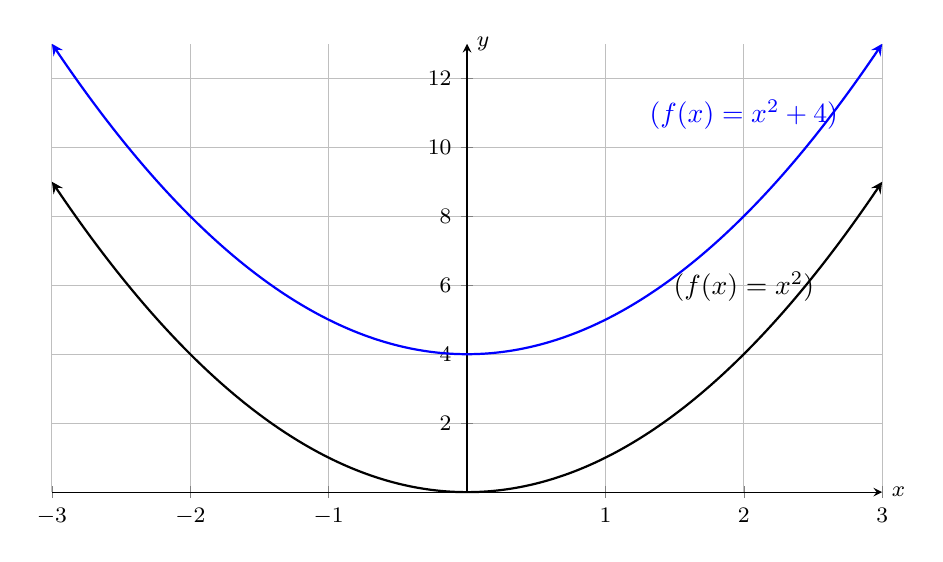
\begin{tikzpicture}
        \begin{axis}[
            my axis style,
            width=\textwidth,
            height=0.6\textwidth,
            ylabel=$y$,
            grid
        ]
        
        \addplot[
            domain=-3:3,
            thick,
            black,
            <->
        ]
        {x^2};

        \addplot[
            domain=-3:3,
            thick,
            blue,
            <->
        ]
        {x^2 + 4};


        \fill[
            black
        ];


        \node[label={90:{\textcolor{blue}{($f(x) = x^2 + 4$)}}},circle,inner sep=2pt] at (axis cs:2,10) {};
        \node[label={90:{\textcolor{black}{($f(x) = x^2$)}}},circle,inner sep=2pt] at (axis cs:2,5) {};
     

        \end{axis}
        \end{tikzpicture}
    \end{center}


\begin{center}
        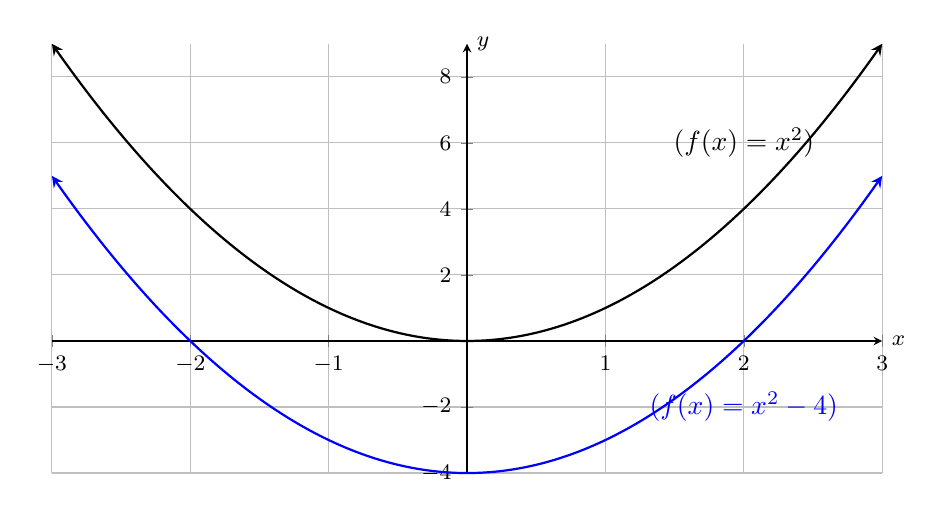
\begin{tikzpicture}
        \begin{axis}[
            my axis style,
            width=\textwidth,
            height=0.58\textwidth,
            ylabel=$y$,
            grid
        ]
        

        \addplot[
            domain=-3:3,
            thick,
            black,
            <->
        ]
        {x^2};

        \addplot[
            domain=-3:3,
            thick,
            blue,
            <->
        ]
        {x^2 - 4};

        \fill[
            black
        ];


        \node[label={90:{\textcolor{blue}{($f(x) = x^2 - 4$)}}},circle,inner sep=2pt] at (axis cs:2,-3) {};
        \node[label={90:{\textcolor{black}{($f(x) = x^2$)}}},circle,inner sep=2pt] at (axis cs:2,5) {};
     

        \end{axis}
        \end{tikzpicture}
    \end{center}

\newpage

\textbf{\large{1. Horizontal Shifting (Ex : $f(x) = \sqrt{x} )$}}

\begin{center}
        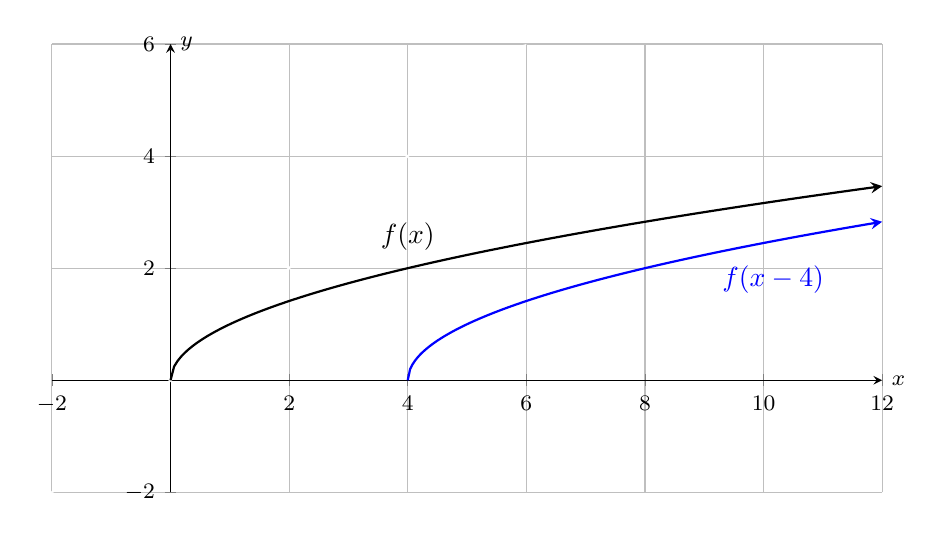
\begin{tikzpicture}
        \begin{axis}[
            my axis style,
            width=\textwidth,
            height=0.6\textwidth,
            ylabel=$y$,
            grid
        ]

        \addplot[
            domain=-2:6,
            thick,
            white,
            ->
        ]
        {x};
        
        \addplot[
            domain=0:12,
            thick,
            black,
            ->
        ]
        {sqrt(x)};

        \addplot[
            domain=4:12,
            thick,
            blue,
            ->
        ]
        {sqrt(x - 4)};


        \fill[
            black
        ];

        \node[label={0:{\textcolor{blue}{$f(x - 4)$}}},circle,inner sep=2pt] at (axis cs:9,1.8) {};
        \node[label={90:{\textcolor{black}{$f(x)$}}},circle,inner sep=2pt] at (axis cs:4,2) {};


        \end{axis}
        \end{tikzpicture}
    \end{center}

\begin{center}
        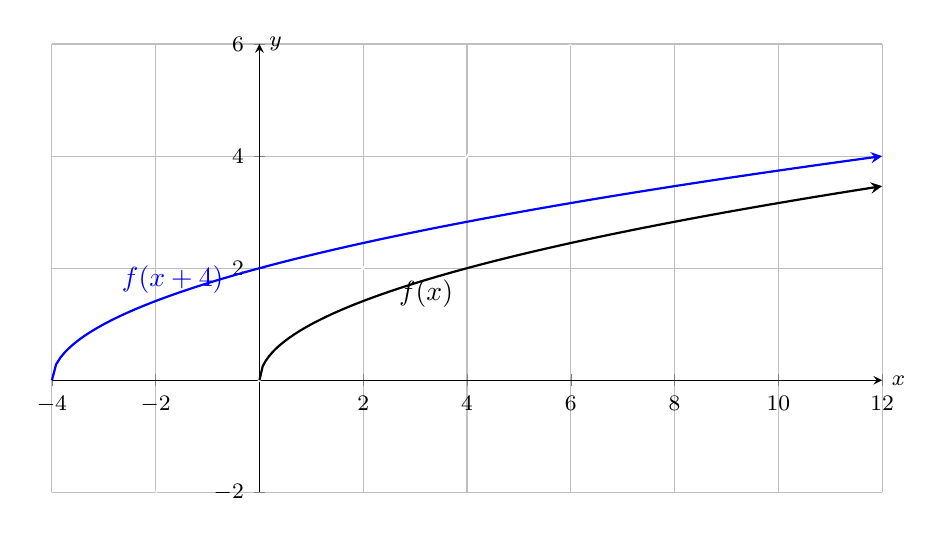
\begin{tikzpicture}
        \begin{axis}[
            my axis style,
            width=\textwidth,
            height=0.6\textwidth,
            ylabel=$y$,
            grid
        ]

        \addplot[
            domain=-2:6,
            thick,
            white,
            ->
        ]
        {x};
        
        \addplot[
            domain=0:12,
            thick,
            black,
            ->
        ]
        {sqrt(x)};

        \addplot[
            domain=-4:12,
            thick,
            blue,
            ->
        ]
        {sqrt(x + 4)};


        \fill[
            black
        ];

        \node[label={0:{\textcolor{blue}{$f(x + 4)$}}},circle,inner sep=2pt] at (axis cs:-3,1.8) {};
        \node[label={120:{\textcolor{black}{$f(x)$}}},circle,inner sep=2pt] at (axis cs:4,1) {};


        \end{axis}
        \end{tikzpicture}
    \end{center}

    \newpage

\textbf{\large{1. Reflecting (Ex : $f(x) = \sqrt{x} )$}}

\begin{center}
        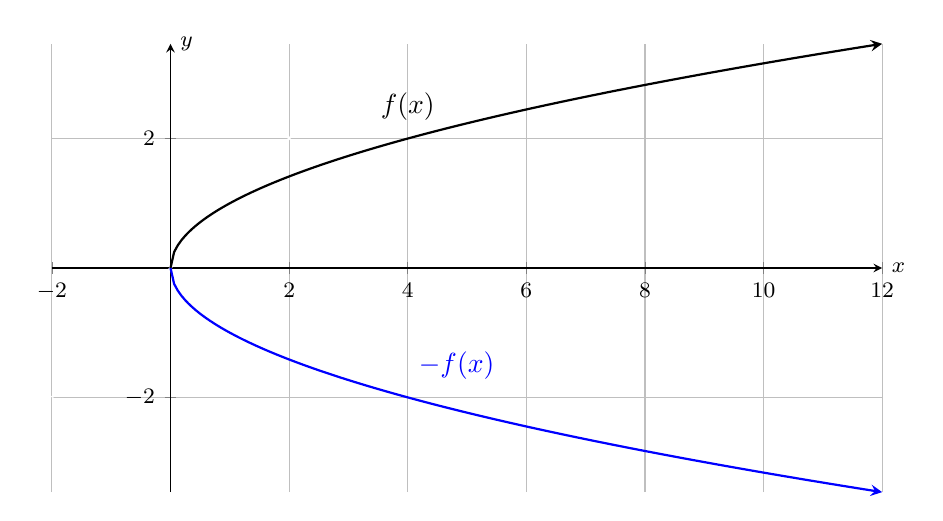
\begin{tikzpicture}
        \begin{axis}[
            my axis style,
            width=\textwidth,
            height=0.6\textwidth,
            ylabel=$y$,
            grid
        ]

        \addplot[
            domain=-2:3,
            thick,
            white,
            ->
        ]
        {x};
        
        \addplot[
            domain=0:12,
            thick,
            black,
            ->
        ]
        {sqrt(x)};

        \addplot[
            domain=0:12,
            thick,
            blue,
            ->
        ]
        {-sqrt(x)};


        \fill[
            black
        ];

        \node[label={80:{\textcolor{blue}{$-f(x)$}}},circle,inner sep=2pt] at (axis cs:4,-2) {};
        \node[label={90:{\textcolor{black}{$f(x)$}}},circle,inner sep=2pt] at (axis cs:4,2) {};


        \end{axis}
        \end{tikzpicture}
    \end{center}

\begin{center}
        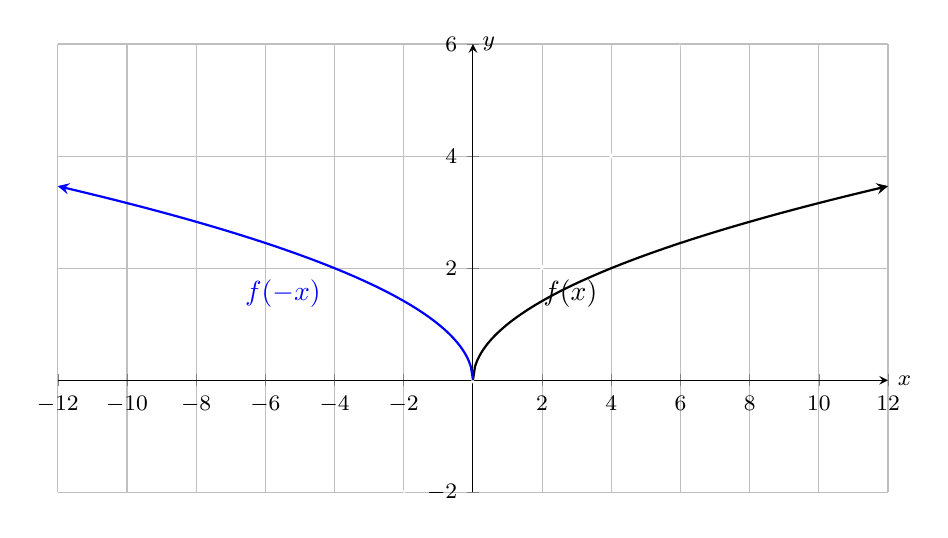
\begin{tikzpicture}
        \begin{axis}[
            my axis style,
            width=\textwidth,
            height=0.6\textwidth,
            ylabel=$y$,
            grid
        ]

        \addplot[
            domain=-2:6,
            thick,
            white,
            ->
        ]
        {x};
        
        \addplot[
            domain=0:12,
            thick,
            black,
            ->
        ]
        {sqrt(x)};

        \addplot[
            domain=-12:0,
            thick,
            blue,
            <-
        ]
        {sqrt(-x)};


        \fill[
            black
        ];

        \node[label={120:{\textcolor{blue}{$f(-x)$}}},circle,inner sep=2pt] at (axis cs:-4,1) {};
        \node[label={120:{\textcolor{black}{$f(x)$}}},circle,inner sep=2pt] at (axis cs:4,1) {};


        \end{axis}
        \end{tikzpicture}
    \end{center}

    \newpage

    \textbf{\large{1. Vertical Compression \& Stretching (Ex : $f(x) = x^2 )$}}

\begin{center}
        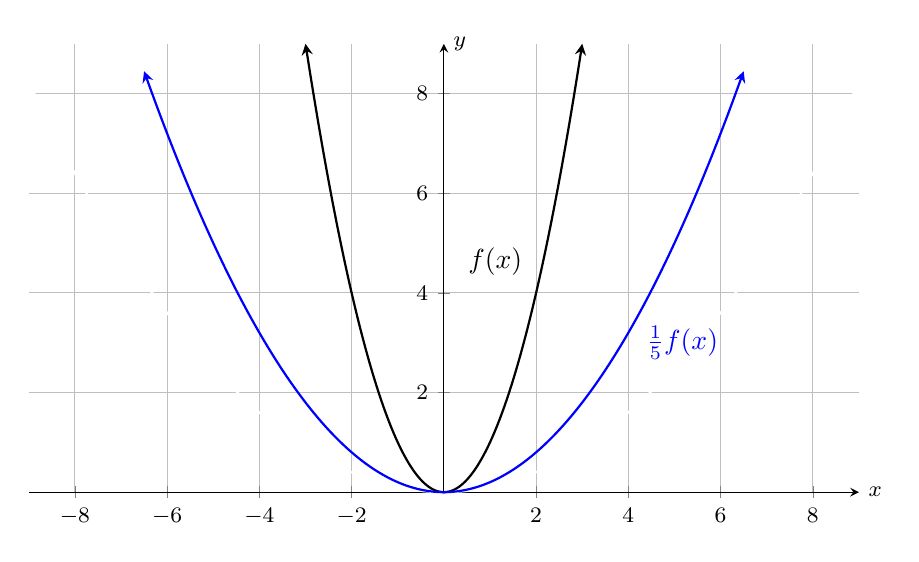
\begin{tikzpicture}
        \begin{axis}[
            my axis style,
            width=\textwidth,
            height=0.6\textwidth,
            ylabel=$y$,
            grid
        ]

        \addplot[
            domain=-9:9,
            thick,
            white,
            <->
        ]
        {0.10*x^2};
        
        \addplot[
            domain=-3:3,
            thick,
            black,
            <->
        ]
        {x^2};

        \addplot[
            domain=-6.5:6.5,
            thick,
            blue,
            <->
        ]
        {0.20*x^2};


        \fill[
            black
        ];


        \node[label={0:{\textcolor{blue}{$\frac{1}{5}f(x)$}}},circle,inner sep=2pt] at (axis cs:4,3) {};
        \node[label={120:{\textcolor{black}{$f(x)$}}},circle,inner sep=2pt] at (axis cs:2,4) {};

        \end{axis}
        \end{tikzpicture}
    \end{center}

\begin{center}
        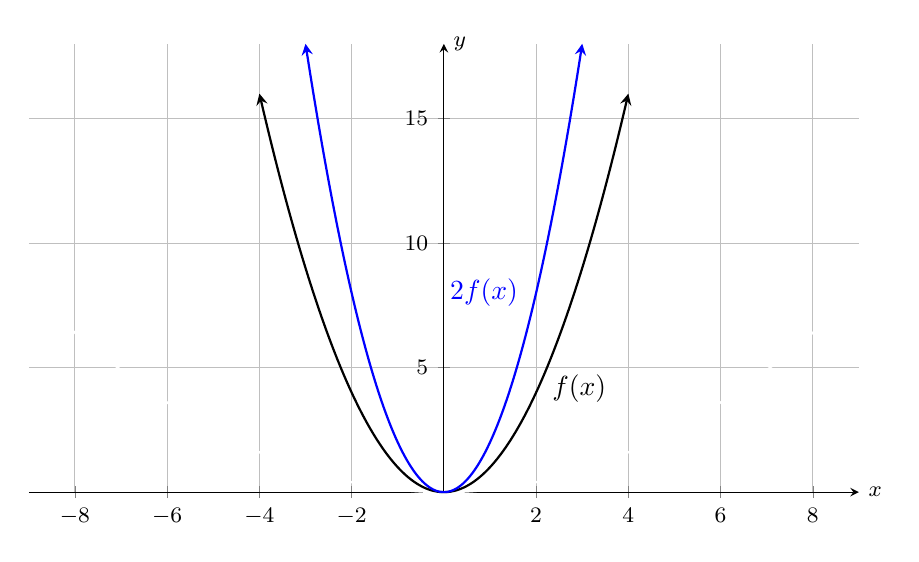
\begin{tikzpicture}
        \begin{axis}[
            my axis style,
            width=\textwidth,
            height=0.6\textwidth,
            ylabel=$y$,
            grid
        ]

        \addplot[
            domain=-9:9,
            thick,
            white,
            <->
        ]
        {0.10*x^2};
        
        \addplot[
            domain=-4:4,
            thick,
            black,
            <->
        ]
        {x^2};

        \addplot[
            domain=-3:3,
            thick,
            blue,
            <->
        ]
        {2*x^2};


        \fill[
            black
        ];


        \node[label={40:{\textcolor{black}{$f(x)$}}},circle,inner sep=2pt] at (axis cs:2,3) {};
        \node[label={180:{\textcolor{blue}{$2f(x)$}}},circle,inner sep=2pt] at (axis cs:2,8) {};

        \end{axis}
        \end{tikzpicture}
    \end{center}

    \newpage

    \textbf{\large{1. Horizontal Stretching \& Compression (Ex : $f(x) = x^2 )$}}

\begin{center}
        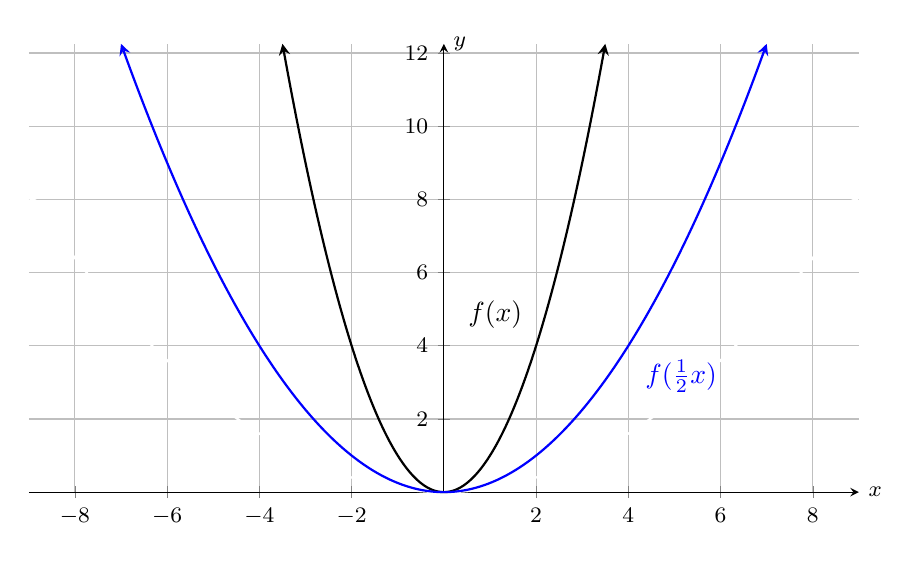
\begin{tikzpicture}
        \begin{axis}[
            my axis style,
            width=\textwidth,
            height=0.6\textwidth,
            ylabel=$y$,
            grid
        ]

        \addplot[
            domain=-9:9,
            thick,
            white,
            <->
        ]
        {0.10*x^2};
        
        \addplot[
            domain=-3.5:3.5,
            thick,
            black,
            <->
        ]
        {x^2};

        \addplot[
            domain=-7:7,
            thick,
            blue,
            <->
        ]
        {0.25*x^2};


        \fill[
            black
        ];


        \node[label={330:{\textcolor{blue}{$f(\frac{1}{2}x)$}}},circle,inner sep=2pt] at (axis cs:4,4) {};
        \node[label={120:{\textcolor{black}{$f(x)$}}},circle,inner sep=2pt] at (axis cs:2,4) {};

        \end{axis}
        \end{tikzpicture}
    \end{center}

\begin{center}
        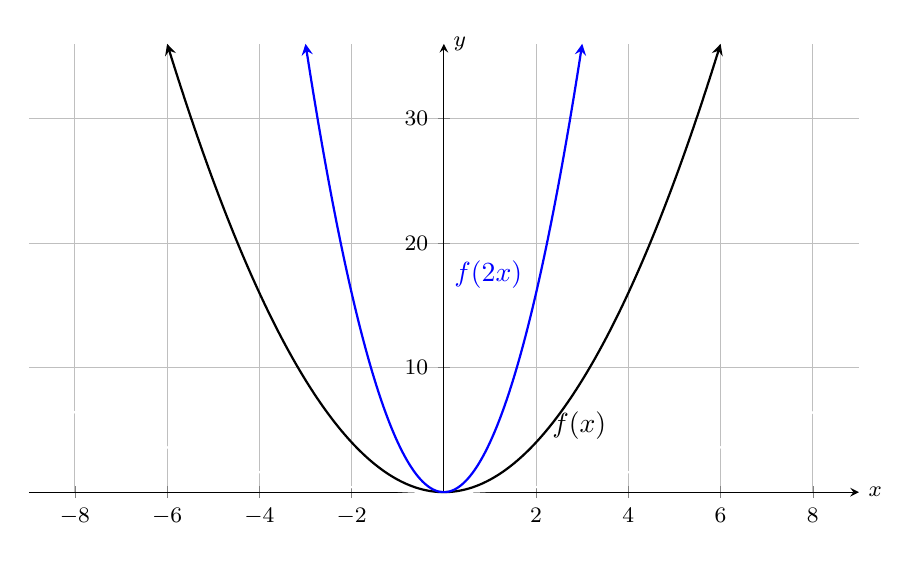
\begin{tikzpicture}
        \begin{axis}[
            my axis style,
            width=\textwidth,
            height=0.6\textwidth,
            ylabel=$y$,
            grid
        ]

        \addplot[
            domain=-9:9,
            thick,
            white,
            <->
        ]
        {0.10*x^2};
        
        \addplot[
            domain=-6:6,
            thick,
            black,
            <->
        ]
        {x^2};

        \addplot[
            domain=-3:3,
            thick,
            blue,
            <->
        ]
        {4*x^2};


        \fill[
            black
        ];


        \node[label={40:{\textcolor{black}{$f(x)$}}},circle,inner sep=2pt] at (axis cs:2,3) {};
        \node[label={120:{\textcolor{blue}{$f(2x)$}}},circle,inner sep=2pt] at (axis cs:2,15) {};

        \end{axis}
        \end{tikzpicture}
    \end{center}



\end{document}















